\chapter{相关技术介绍}
本章概述了相关技术的基础知识,包括Clang和Libclang、自动机、
抽象语法树(AST)以及程序控制流图(CFG),
并探讨了这些技术在编译器设计、代码分析和静态检查中的应用。
其次,本章还对NFA到DFA的转换算法:子集构造法进行了介绍。
\section{Clang和Libclang}
Clang是一款现代化、开源的C/C++编译器前端工具。它由LLVM项目开发,并于2007年首次发布。作为一个强大而灵活的编译器,
Clang在编译速度、代码覆盖率和用户友好性等方面都有着显著的优势。

Clang的由来可以追溯到对现有编译器的不满。传统C/C++编译器(如gcc)的错误报告和诊断信息通常不够详尽和友好,
给开发者带来了很多挑战。由于缺乏语义理解和严格的错误检查,开发者常常需要反复运行代码以找出潜在的问题,十分麻烦。
所以Clang应运而生,旨在解决这些问题并提供更好的开发体验。

Clang的发展历程中,引入了许多创新的特性。首先,Clang采用了模块化的设计,
使得编译器的各个组件可以独立地进行扩展和修改。这种设计使得Clang更加灵活,
并且可以更容易地支持新的语言特性和编译技术。开发者不必下载整个程序,可以选择库中自己所需要的工具,
只使用一部分的编译器的功能,
例如源代码的生成和分析,本工具原型便利用来Clang来获取C语言程序的AST。

其次,Clang具有出色的性能和编译速度。它通过使用先进的编译技术,
如增量编译和即时编译(JIT),在保持高标准的代码质量的同时提高了开发者的效率。
这对于大型项目和需要频繁编译的场景来说非常重要。

此外,Clang还提供了强大的代码静态分析能力。它可以检查代码中的潜在问题,
如空指针解引用和内存泄漏,并提供详细的错误报告和警告信息。
这有助于开发人员在开发过程中尽早发现和修复潜在的bug,提高代码质量和可靠性,也可用于开发de中的代码提示。

作为一个通用的编译器前端工具,Clang不仅支持标准的C和C++语言,
还提供了对其他编程语言的扩展。例如,它支持Objective-C和Objective-C++,使得开发iOS和macOS应用程序也变得更加便捷。
不仅如此,Clang还支持OpenCL和CUDA等并行计算语言,以及一些领域特定语言,对并行编程也有很大帮助。

总而言之,Clang是一个功能强大、高性能且易于使用的C/C++编译器前端工具。
它通过提供详细的错误报告、优化编译速度和支持多种编程语言的扩展,为开发者提供了更好的开发体验和更高效的工作流程。
无论是学习编程还是进行大规模软件开发,Clang都是一个值得考虑的首选工具。\\


Libclang是针对Clang编译器的C语言库接口,旨在为开发者提供一种方便的方式来访问和操作Clang的功能。

Libclang的出现可以追溯到Clang项目的发展。
由于Clang的模块化设计,使得它的各个部分可以被单独使用和扩展。
为了让更多的开发者能够利用Clang的功能,将其核心部分抽离出来,
便开发了独立的C语言库接口,即Libclang。

从设计结构上,Libclang从Clang项目中单独分离出来,作为一个独立的库,并可用于各种编程语言的应用程序的开发。
从具体功能上,Libclang与Clang编译器也有着密切的关系。它是Clang编译器的API接口,允许开发者直接访问Clang的各个部分,
如词法分析、语法分析和语义分析等。通过使用Libclang,开发者可以利用Clang的强大功能,
进行代码分析、生成抽象语法树(AST)以及其他与编译器相关的操作。

随着时间的推移,Libclang得到了广泛的应用和发展。它成为了许多IDE(集成开发环境)和代码编辑器的重要组件,
如Visual Studio Code、Qt Creator和Eclipse等。通过集成Libclang,
这些工具可以提供语法高亮、代码补全、代码导航和代码重构等功能,大大提升了开发者的效率。

Libclang的作用不仅仅局限于开发工具的集成。它还为其他各种代码分析和处理工具提供了强大的支持。
例如,通过使用Libclang,开发者可以编写自定义的静态分析工具,用于检查代码质量、发现潜在的问题和改进代码可读性。
此外,Libclang还被广泛用于生成文档、构建自动化工具和进行代码重构等任务。

总之,Libclang作为Clang编译器的C语言库接口,为开发者提供了一种便捷的方式来访问和操作Clang的功能。
通过集成Libclang,开发者可以利用Clang的强大能力进行代码分析、生成抽象语法树,
并在各种开发工具和自动化工具中实现更高效的开发流程。

本工具原型采用了基于这套c语言接口的 Python binding,它在使用上与c语言接口是基本一致,环境配置也很简单。
\section{自动机}
自动机是一种计算模型,用于描述离散系统的行为和状态转换。它由一组离散的状态和根据输入信息进行状态转换的规则组成。自动机能根据当前状态和输入来决定下一个状态,它可以处理一系列输入并作出相应响应。
以下是对自动机的正式定义\cite{hopcroft2006}:
一个自动机 \( A \) 可以形式化地表示为一个五元组 \( A = (Q, \Sigma, \delta, q_0, F) \),其中:

\begin{itemize}
    \item \textbf{输入字母表(Input Alphabet)} \( \Sigma \):\(\Sigma\) 是一组离散的符号或字母,表示自动机可以接受的输入。每个输入符号都代表一种可能的输入。
    
    \item \textbf{状态集合(Set of States)} \( Q \): \( Q \) 是自动机可能处于的所有状态的集合。每个状态 \( q \in Q \) 代表自动机在某一时间点的状态。
    
    \item \textbf{转移函数(Transition Function)} \( \delta \): \(\delta: Q \times \Sigma \rightarrow Q\) 是一个映射函数,它将当前状态和输入符号映射到下一个状态。它描述了自动机在接收某个输入符号后转移到哪个状态。
    
    \item \textbf{起始状态(Start State)} \( q_0 \): \( q_0 \in Q \) 是自动机开始执行时的初始状态。
    
    \item \textbf{终止状态集合(Set of Final or Accepting States)} \( F \): \( F \subseteq Q \) 是自动机的一组终止状态。当自动机达到终止状态时,它表示自动机已经完成了特定的工作或接受了特定的输入序列。
\end{itemize}

根据自动机的具体类型,可以有不同的变体,例如确定性有限状态机和非确定性有限状态机
。在确定性有限状态机中,对于给定的输入,
每个状态都只有唯一的下一个状态。
而在非确定性有限状态机中,对于给定的输入,一个状态可能有多个下一个状态。

自动机是一种重要的概念,在计算机科学和工程中被广泛应用于编程、软件工程、人工智能和理论计算等领域。
它可以用于建模和解决各种问题,如自动控制系统、编译器、语言处理、网络协议和人工智能算法等。

下面是一个简单的确定性有限状态机的例子,用来检测二进制数字是否是3的倍数。
这个 DFA 会有三个状态,分别对应二进制数字模 3 的余数为 0、1 和 2 的情况。

状态定义:
\begin{itemize}
    \item $S_0$: 当前数模 3 的余数为 0。
    \item $S_1$: 当前数模 3 的余数为 1。
    \item $S_2$: 当前数模 3 的余数为 2。
\end{itemize}
转换规则:
\begin{center}
    \begin{tabular}{c|c|c}
        状态 & 读取 0 & 读取 1 \\
        \hline
        $S_0$ & $S_0$ & $S_1$ \\
        $S_1$ & $S_2$ & $S_0$ \\
        $S_2$ & $S_1$ & $S_2$ \\
    \end{tabular}
\end{center}
初始状态和接受状态都是$S_0$(因为模 3 余数为 0 表示该数是 3 的倍数)

图\ref{fig:DFA状态转移图}是该DFA的状态转移图:
\begin{figure}[htbp]
	\centering
	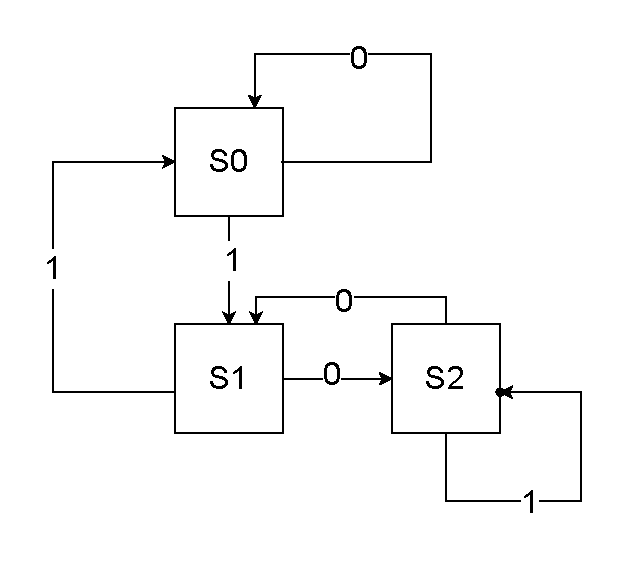
\includegraphics[width=0.7\textwidth]{pictures/DFA状态转移图.pdf}
	\caption{DFA状态转移图}
	\label{fig:DFA状态转移图}
\end{figure}
作者可以用这个状态转换图来实现一个简单的有限状态机,用于检测二进制数是否是 3 的倍数。
例如,考虑二进制数字 "110"(对应十进制的 6):
\begin{itemize}
	\item 初始状态:$ S_0 $
	\item 读取第一个字符 '1':状态从$ S_0 $变为$ S_1 $
	\item 读取第二个字符 '1':状态从$ S_1 $变为$ S_0 $
	\item 读取第三个字符 '0':状态从$ S_0 $变为$ S_0 $
\end{itemize}
最终状态是$ S_0 $,因此 "110" 是 3 的倍数。

\subsection{确定有限状态自动机}
确定性有限状态机(Deterministic Finite State Machine,DFA)是自动机的一种常见类型。
DFA具有以下几个特征和工作原理:
\begin{enumerate}
	\item 确定性转移: 对于给定的输入符号和当前状态,在DFA中每个状态只对应一个确定的下一个状态。
 也就是说,对于任何时刻,DFA可以根据当前状态和输入符号直接确定下一个状态,没有歧义或多义性。
	\item 状态转移: DFA通过状态转移来处理输入序列。从起始状态开始,根据输入符号,
 使用转移函数δ将DFA移动到下一个状态,然后继续接受下一个输入符号,如此往复,直到结束。
	\item 终止状态: 当DFA达到一个终止状态时,它表示DFA已经完成了特定的任务或接受了特定的输入序列。
 终止状态可以是一个或多个,DFA的任务和行为取决于达到哪些终止状态。
	\item 接受和拒绝: 执行结束后,如果DFA的最终状态属于终止状态集合F,则它接受输入序列;
 否则,它拒绝输入序列。
	\item 状态转移图: DFA的行为通常用状态转移图(State Transition Diagram)表示。
 状态用节点表示,转移用箭头表示。起始状态通常有一个入口箭头指向它,终止状态可能通过双圈或其他标记来表示。
\end{enumerate}
DFA是一种简单且易于理解的自动机模型。由于其确定性的特征,DFA在模式匹配、语法分析、词法分析和编译器设计等领域中得到广泛应用。
DFA可以用于验证、识别和处理各种类型的输入,如编程语言的关键字、标识符或语法规则等。它是构建更复杂自动机的基础,如正则表达式引擎和有限状态机网络。
\subsection{非确定有限状态自动机}
非确定性有限状态机(Nondeterministic Finite State Machine,NFA)是自动机的另一种常见类型,
与确定性有限状态机(DFA)相比,它具有一些特殊的特征和行为。

NFA具有以下几个特征和工作原理:
\begin{enumerate}
	\item 非确定性转移: 在NFA中,对于给定的输入符号和当前状态,一个状态可以对应多个可能的下一个状态。
 这样的非确定性转移使得NFA在处理输入时具有更大的灵活性。
	\item ε-转移(ε-Transition): NFA可以进行ε-转移,即在不消耗输入符号的情况下从一个状态跳转到另一个状态。
 这样的转移可以让NFA同时处于多个状态。
	\item 状态转移: 与DFA类似,NFA通过状态转移来处理输入序列。
 根据当前状态和输入符号,NFA使用转移函数δ将其移动到下一个状态集合。
	\item 终止状态: 当NFA中的任何一个状态达到终止状态时,它表示NFA已经完成了特定的任务或接受了特定的输入序列。
	\item 接受和拒绝: NFA根据其终止状态的集合来接受或拒绝输入序列。如果在执行结束时,
 NFA的最终状态中至少有一个状态属于终止状态集合F,则它接受输入序列;否则,它拒绝输入序列。
    \item 状态转移图: NFA的行为通常用状态转移图表示,其中状态用节点表示,转移用箭头表示。
    不同于DFA,NFA的转移箭头可以具有ε-转移和多个目标状态。
\end{enumerate}
NFA相比于DFA具有更大的灵活性和表达能力。由于其非确定性的特征,NFA在正则表达式引擎、模式匹配、语言处理和编译器设计等领域中得到广泛应用。
NFA通常被用作构建更复杂自动机模型的基础,如非确定性推导树和确定性有限状态机(DFA)。

本工具原型中,根据生成的AST,首先生成的只是相应的NFA,但是要想准确定位错误,能够将某一个状态具体对应到代码的某一段,还需要将NFA转换成
DFA,对于这一转换,本工具原型采用的是子集构造法。
\subsection{子集构造法}
子集构造法(Subset Construction Method)是一种将非确定有限状态自动机(NFA)转换为等价的确定有限状态自动机(DFA)的算法。
该算法的基本思想是根据NFA的状态集合构造DFA的状态集合,并在状态转移函数中处理相应的转移。

以下是子集构造法的大体步骤:
\begin{enumerate}
	\item  初始状态:
 从NFA的初始状态开始,构造DFA的初始状态,即将初始状态作为DFA的初始状态。
    \item  状态转移:
对于每个DFA状态和每个输入符号,找到对应的NFA状态集合。
对于该输入符号,将NFA状态集合进行ε-闭包处理,即找到所有通过ε(空转移)可以到达的状态。
将得到的ε-闭包状态集合作为DFA状态的转移目标,并根据输入符号找到相应的转移。
    \item  状态集合构建:
对于每个新构造的DFA状态,重复第二步骤,直到没有新的状态可以构造。
    \item  判断接受状态:
根据NFA的接受状态集合来判断DFA的接受状态。
如果DFA的状态集合中包含任何一个NFA的接受状态,则将该DFA状态标记为接受状态。
\end{enumerate}
通过使用子集构造法,可以将NFA转换为等价的DFA。


\section{抽象语法分析树}
抽象语法树(Abstract Syntax Tree,AST)是一个用于代表程序代码层次结构的树状数据结构。许多编译器,解释器以及静态分析工具都是以此为
开发基础。AST通过将代码语法拆解成了抽象的语法树结构,提供了一种以层次化,结构化理解和处理代码的方式。代码提示,格式化,debug工具,或者自动生成序列化代码等等,这些功能的开发都需要语法树里面的信息。
AST将代码中的各个元素(如表达式Expression,语句Statement,声明Declaration等)转化为语法树中的节点,而节点之间通过父子关系建立连接。
通常情况下,AST的根节点表示整个代码文件,然后每个语法结构(如函数、循环、条件语句等)都成为根节点的子节点。子节点可以继续有自己的子节点,以此类推,形成一个树状结构。

例如,对于一段表示欧几里得算法的C语言代码:\\
\begin{figure}[htbp]
    \centering
\begin{minipage}{4cm}
\begin{lstlisting}[language=c++]
while b ≠ 0:
    if a > b:
        a := a - b
    else:
        b := b - a
return a
\end{lstlisting}
\end{minipage}

\end{figure}


其AST的每一棵子树都会对应语句中的某一部分,
如while子树将会有condition和body两个子树,condition中包含了用于判断的表达式,body则是包含了判断为true时
需要执行的内容,如图\ref{fig:AST树}所示:
\begin{figure}[htbp]
	\centering
	\includegraphics[width=0.6\textwidth]{pictures/AST树.png}
	\caption{AST树}
	\label{fig:AST树}
\end{figure}


Clang的抽象语法树(AST)类层次结构主要分为以下几大类,每一类都代表不同的语言构造和抽象概念。

第一类是AST Context(AST上下文),它管理类型和声明的内存池。

第二类是Declaration(声明),代表各种声明,如变量声明、函数声明等。它的子类包括具名声明(NamedDecl),表示有名字的声明,如变量、函数、类型别名;和类型声明(TypeDecl),表示类、结构体、枚举等类型。具名声明的子类有值声明(ValueDecl),表示变量和函数等具有值的声明,以及类型声明(TypeDecl),表示类型别名和标签类型。模板声明(TemplateDecl)也属于这一类。

第三类是DeclContext(声明上下文),它是可以包含其他声明的上下文,如命名空间、记录、函数体等。命名空间声明(NamespaceDecl)和记录声明(RecordDecl)是DeclContext的子类。

第四类是Statement(语句),代表各种语句,如表达式语句、控制流语句等。它的子类包括表达式(Expr)、复合语句(CompoundStmt,表示包含多条语句的语句块)、if语句(IfStmt)、for循环语句(ForStmt)、while循环语句(WhileStmt)和return语句(ReturnStmt)。

最后一类是Type(类型),表示具体的数据类型,如int、char等。

在Clang生成的AST中,其根节点是TranslationUnitDecl,代表了一个C语言程序,可以从此开始遍历整个AST树,也可以获取已解析的的标识符表。
Clang的AST节点并没有一个共同的“NODE”基类,大部分AST节点派生自 Type、 Decl、 DeclContext 或Stmt,还有一些节点属于自己的特定结构。
因此,要遍历完整的AST,需要从TranslationUnitDecl开始,然后递归地遍历从该节点可以到达的所有内容,并针对每种特定节点类型对这一信息进行编码。
该算法被编码在一个RecursiveASTVisitor中。
\section{程序控制流图}
程序控制流图程序控制流图(Program Control Flow Graph)是一种用于表示程序执行流程的图形结构。
它描述了程序中不同语句之间的控制流结构。
程序控制流图有助于可视化和分析程序的结构,并在软件工程中广泛应用于代码分析、特别是数据流分析相关的技术。

一个程序控制流图由以下几个基本元素组成:
\begin{itemize}
	\item 基本块(Basic Block):基本块是程序控制流图的基本单元,它是一组语句的顺序执行序列。基本块内部没有分支和跳转语句,只有一个进入点和一个退出点。基本块可以包含多行代码,但通常被简化为单个语句。
    \item 控制边(Control Edge):控制边用于表示程序控制的转移关系。它连接了控制流图中的不同基本块,指示程序的执行流从一个基本块转移到另一个基本块。控制边也可以表示条件分支、循环结构和其他控制转移。
    \item 进入点(Entry Point):进入点是控制流图中的起始点,它标识程序的入口,表示程序开始执行的位置。
    \item 退出点(Exit Point):退出点是控制流图中的终止点,它标识程序的出口,表示程序结束执行的位置。
\end{itemize}

从AST生成CFG的过程涉及根据语法结构中的控制流语句
(如条件语句、循环语句等)来构建控制流。通过遍历AST树并识别程序流控制相关的节点,
工具原型可以建立一个CFG来表示程序中的控制流。

举个例子,考虑以下简单的代码片段,一个main函数中包含了一个while循环:\\

\begin{figure}[htbp]
    \centering
\begin{minipage}{4cm}
\begin{lstlisting}[language=c++]
int main() {
    int i = 0;
    while (i < 10) {
        i++;
    }
    return 0;
}
\end{lstlisting}
\end{minipage}
\end{figure}

首先,编译器或解析器会将这段代码转化为AST,如下图所示。

\begin{tikzpicture}
\Tree
[.TranslationUnit
    [.FunctionDeclaration(main)
        [.CompoundStatement
            [.VariableDeclaration ]
            [.WhileStatement 
                [.Condition ]
                [.CompoundStatement 
                    [.ExpressionStatement ]
                ]
            ]
            [.ReturnStatement ]
        ]
    ] 
]

\end{tikzpicture}
\begin{comment}
\begin{figure}[htbp]
	\centering
	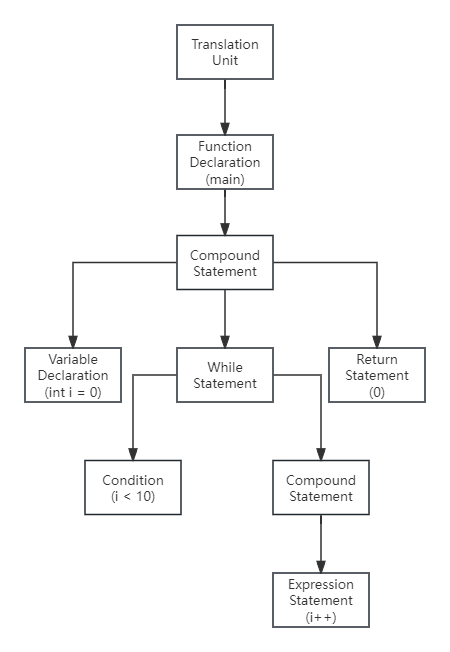
\includegraphics[width=0.5\textwidth]{pictures/AST例子.png}
	\caption{AST例子}
	\label{fig:AST例子}
\end{figure}
\end{comment}

然后,通过分析AST,工具原型可以构建一个简单的CFG来表示控制流,如图\ref{fig:cfg的例子}所示。





\begin{figure}[htbp]
	\centering
	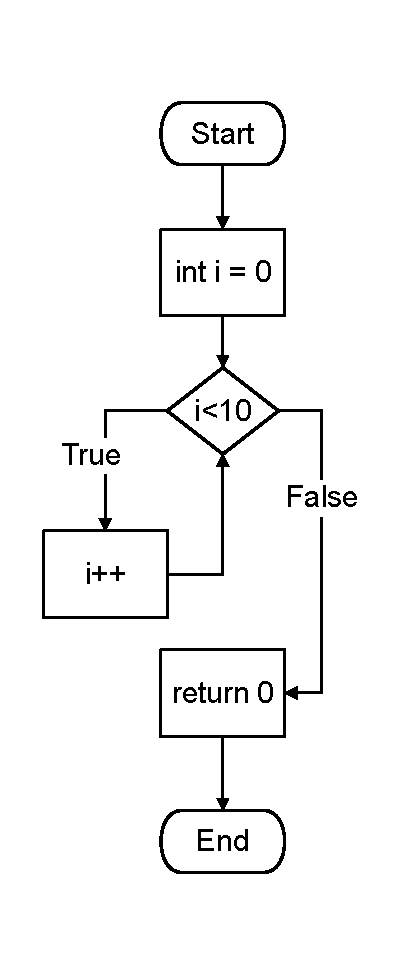
\includegraphics[width=0.3\textwidth]{pictures/cfg例子.pdf}
	\caption{cfg的例子}
	\label{fig:cfg的例子}
\end{figure}




值得注意的是,在本工具原型中,作者关注的主要是由日志函数,
所以,对于一些不包含日志的语句或者结构简单的语句,可以当作空语句处理
,这有助于简化CFG的整体结构。
\section{本章小结}
本章详细介绍了工具原型所运用的各类技术,包括 Clang 和 Libclang,用于生成和解析 C语言 程序的抽象语法树(AST),以及自动机(NFA 和 DFA)的基本概念及其在程序控制流图中的应用。最后,本文阐述了抽象语法树和程序控制流图的基本原理和结构。

